\documentclass[10 pt]{article}

\usepackage[utf8x]{inputenc}
\usepackage{dsfont}
\usepackage{amsthm}
\usepackage{amsfonts}
\usepackage{tensor}
\usepackage{mathtools}
\usepackage[T1]{fontenc}
%\usepackage[spanish]{babel}
\usepackage[cm]{fullpage}
\usepackage{graphicx}
\usepackage{float}
\usepackage{bm}
\usepackage{setspace}
\usepackage{enumitem}
\usepackage{mdwlist}
\usepackage{parskip}
\usepackage{listings}
\usepackage{color}
%\usepackage{epstopdf}
\usepackage{tikz,datatool}
\usepackage{hyperref}

\newcommand{\HRule}{\rule{\linewidth}{0.5mm}}

\AtBeginDocument{
  \let\myThePage\thepage
  \renewcommand{\thepage}{\oldstylenums{\myThePage}}
}

\newcommand{\gra}{$^\text{o}$}
\newcommand{\dif}{\text{d}}
\newcommand{\avg}[1]{\left\langle #1 \right\rangle}
\newcommand{\ket}[1]{\left| #1 \right\rangle}
\newcommand{\bra}[1]{\left\langle #1 \right|}
\newcommand{\bket}[2]{\left\langle #1 \middle| #2 \right\rangle}
\newcommand{\der}[2]{\frac{\text{d} #1}{\text{d} #2}}
\newcommand{\prt}[2]{\frac{\partial #1}{\partial #2}}
\newcommand{\dert}[3]{\frac{\text{d}^#3 #1}{\text{d} #2^#3}}
\newcommand{\prtt}[3]{\frac{\partial^#3 #1}{\partial #2^#3}}
\newcommand{\dl}{\mathcal{L}}
\newcommand{\dha}{\mathcal{H}}
\newcommand{\vol}{\text{vol}}
\renewcommand{\vec}[1]{\pmb{#1}}

\newenvironment{algo}[1]
{  \begin{center}
   \mbox{
       \begin{minipage}{\textwidth}
           \begin{tabbing}
           \settabs
            #1
           \end{tabbing}
        \end{minipage}
    }
    \end{center}
}{}
\newcommand{\settabs}{mmm\=mmm\=mmm\=mmm\=mmm\=mmm\=\kill}

\DeclarePairedDelimiter\ceil{\lceil}{\rceil}
\DeclarePairedDelimiter\floor{\lfloor}{\rfloor}

\definecolor{mygray}{rgb}{0.4,0.4,0.4}
\definecolor{mygreen}{rgb}{0,0.5,0.25}
\definecolor{myorange}{rgb}{1.0,0.4,0}

\definecolor{clock0}{cmyk}{1,0,0,0}
\definecolor{clock1}{cmyk}{1,1,0,0}
\definecolor{clock2}{cmyk}{0,1,0,0}
\definecolor{clock3}{cmyk}{0,1,1,0}
\definecolor{clock4}{cmyk}{1,0,1,0}
\definecolor{clock5}{cmyk}{1,1,1,0}
\definecolor{clock6}{cmyk}{0,0,1,0}
\definecolor{clock7}{cmyk}{0,0,0,0.1}

\begin{document}

\lstset{
language=C++,
basicstyle=\ttfamily\color{black},
commentstyle=\color{mygray}\ttfamily,
frame=single,
numbers=left,
numbersep=5pt,
numberstyle=\tiny\color{mygray}\ttfamily,
keywordstyle=\color{mygreen}\ttfamily,
showspaces=false,
showstringspaces=false,
stringstyle=\color{myorange}\ttfamily,
tabsize=2,
emph={double,uint8_t,uint16_t,uint32_t,uint64_t,int8_t,int16_t,int32_t,int64_t},
emphstyle={\color{blue}\ttfamily}
}

\begin{center}
  \Large \textsc{Week 3: Monte Carlo simulation of Hard disks in the NVT ensemble}
\end{center}

\begin{center}
  \large \textsc{Francisco García Flórez}
\end{center}

\section{Hard spheres in two dimensions}

\subsection{Packing fraction}

Firstly, we will study rectangular and hexagonal lattices in two dimensions and compute their packing fractions. In the following representation we have plotted the initial configuration for these two systems:

\begin{figure}[H]
  \begin{center}
    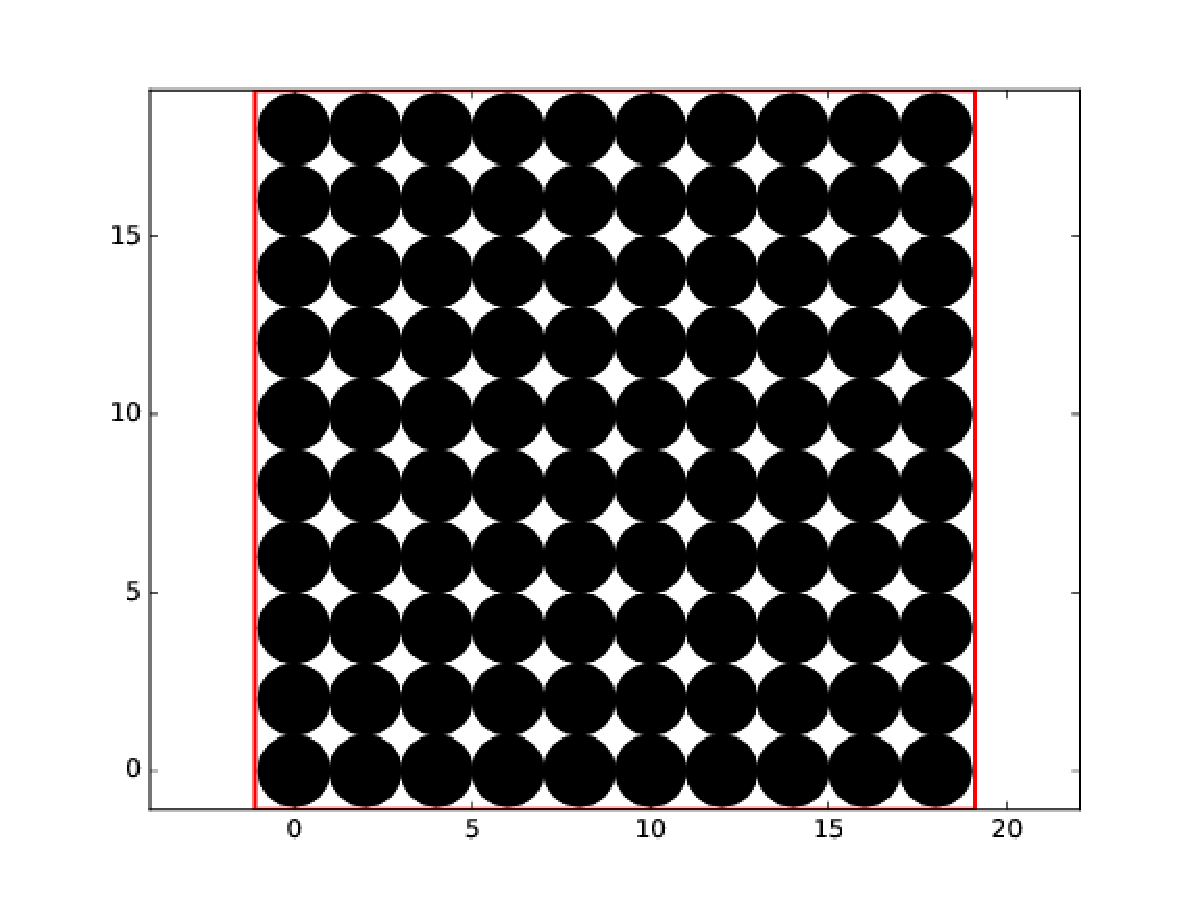
\includegraphics[width=0.45\textwidth]{../graphs/rectangular.pdf}
    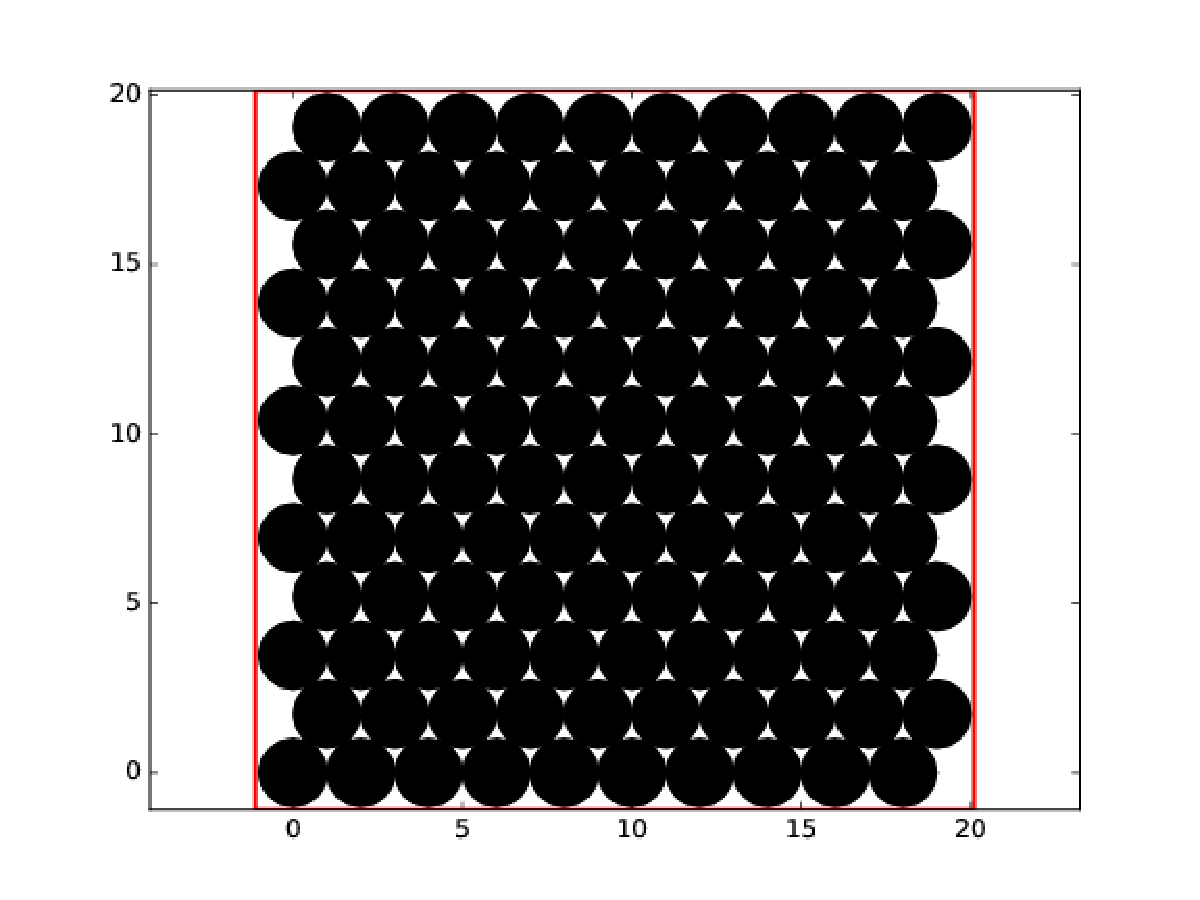
\includegraphics[width=0.45\textwidth]{../graphs/hexagonal.pdf}
    \caption{Graphical representation of a rectangular lattice (left) and an hexagonal lattice (right). Boundary limits are shown by a red line.}
  \end{center}
\end{figure}

The packing fraction is defined as the ratio of one unit cell's volume and the occupied volume of every particle inside. For the rectangular lattice is straightforward, because the unit cell is just the square around one sphere. Thus, the packing fraction $\eta$ is

$$ \eta = \frac{\pi r^2}{4 r^2} = \frac{\pi}{4} \sim 0.7854 $$

For the hexagonal lattice though, the unit cell contains some part of multiple spheres, but following a similar procedure we can get

$$ \eta = \frac{\pi}{2\sqrt{3}} \sim 0.9069 $$

As expected, the hexagonal lattice is significantly denser.

\subsection{Melting point}

Now, the packing fraction is directly related to the solid-liquid transition in these systems, so let's compute when it happens as a function of $\eta$. For that, we will compute $R^2(N)$ for each particle, average it over all particles to get $\avg{R^2(N)}$ and then take only the last value so it only depends on $\eta$: $\avg{R^2(\eta)}$.

In the following plot we are representing this value for multiple values of the packing fraction:

\begin{figure}[H]
  \begin{center}
    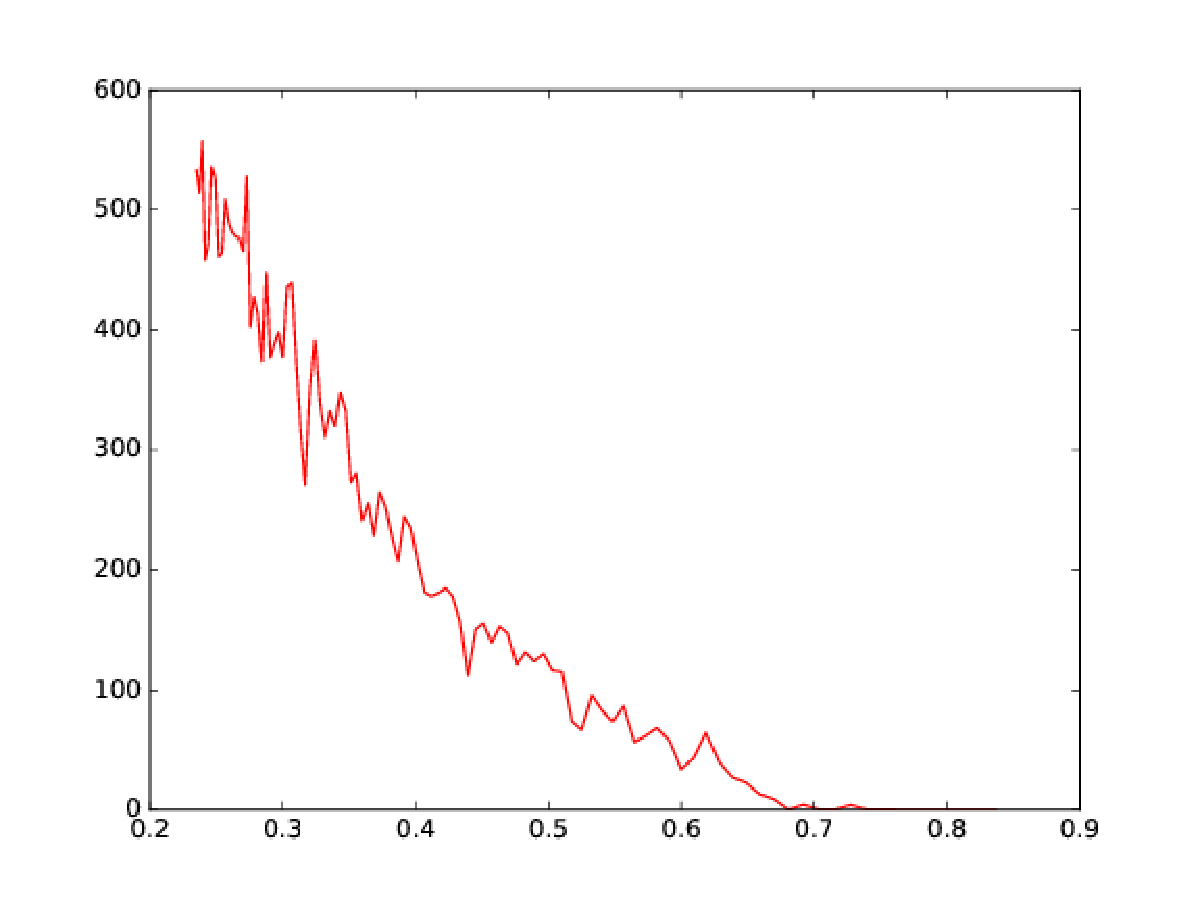
\includegraphics[width=0.7\textwidth]{../graphs/hexa-melting.pdf}
    \caption{Graphical representation of $\avg{R^2(\eta)}$ for an hexagonal lattice.}
  \end{center}
\end{figure}

It is really easy to see from this plot that the value of $\eta_*$ in the transition is around $\sim 0.67$, as in this point $\avg{R^2(\eta)}$ changes from being constant and almost zero to increase linearly-looking for $\eta < \eta_*$. There is a change in slope at $\eta \sim 0.4$, maybe because of another less significant transition.

\section{Hard spheres in three dimensions}

In this case we will consider the simple cubic (SC) lattice and the face-centered cubic (FCC) lattice, as we can see in the following representation.

\begin{figure}[H]
  \begin{center}
    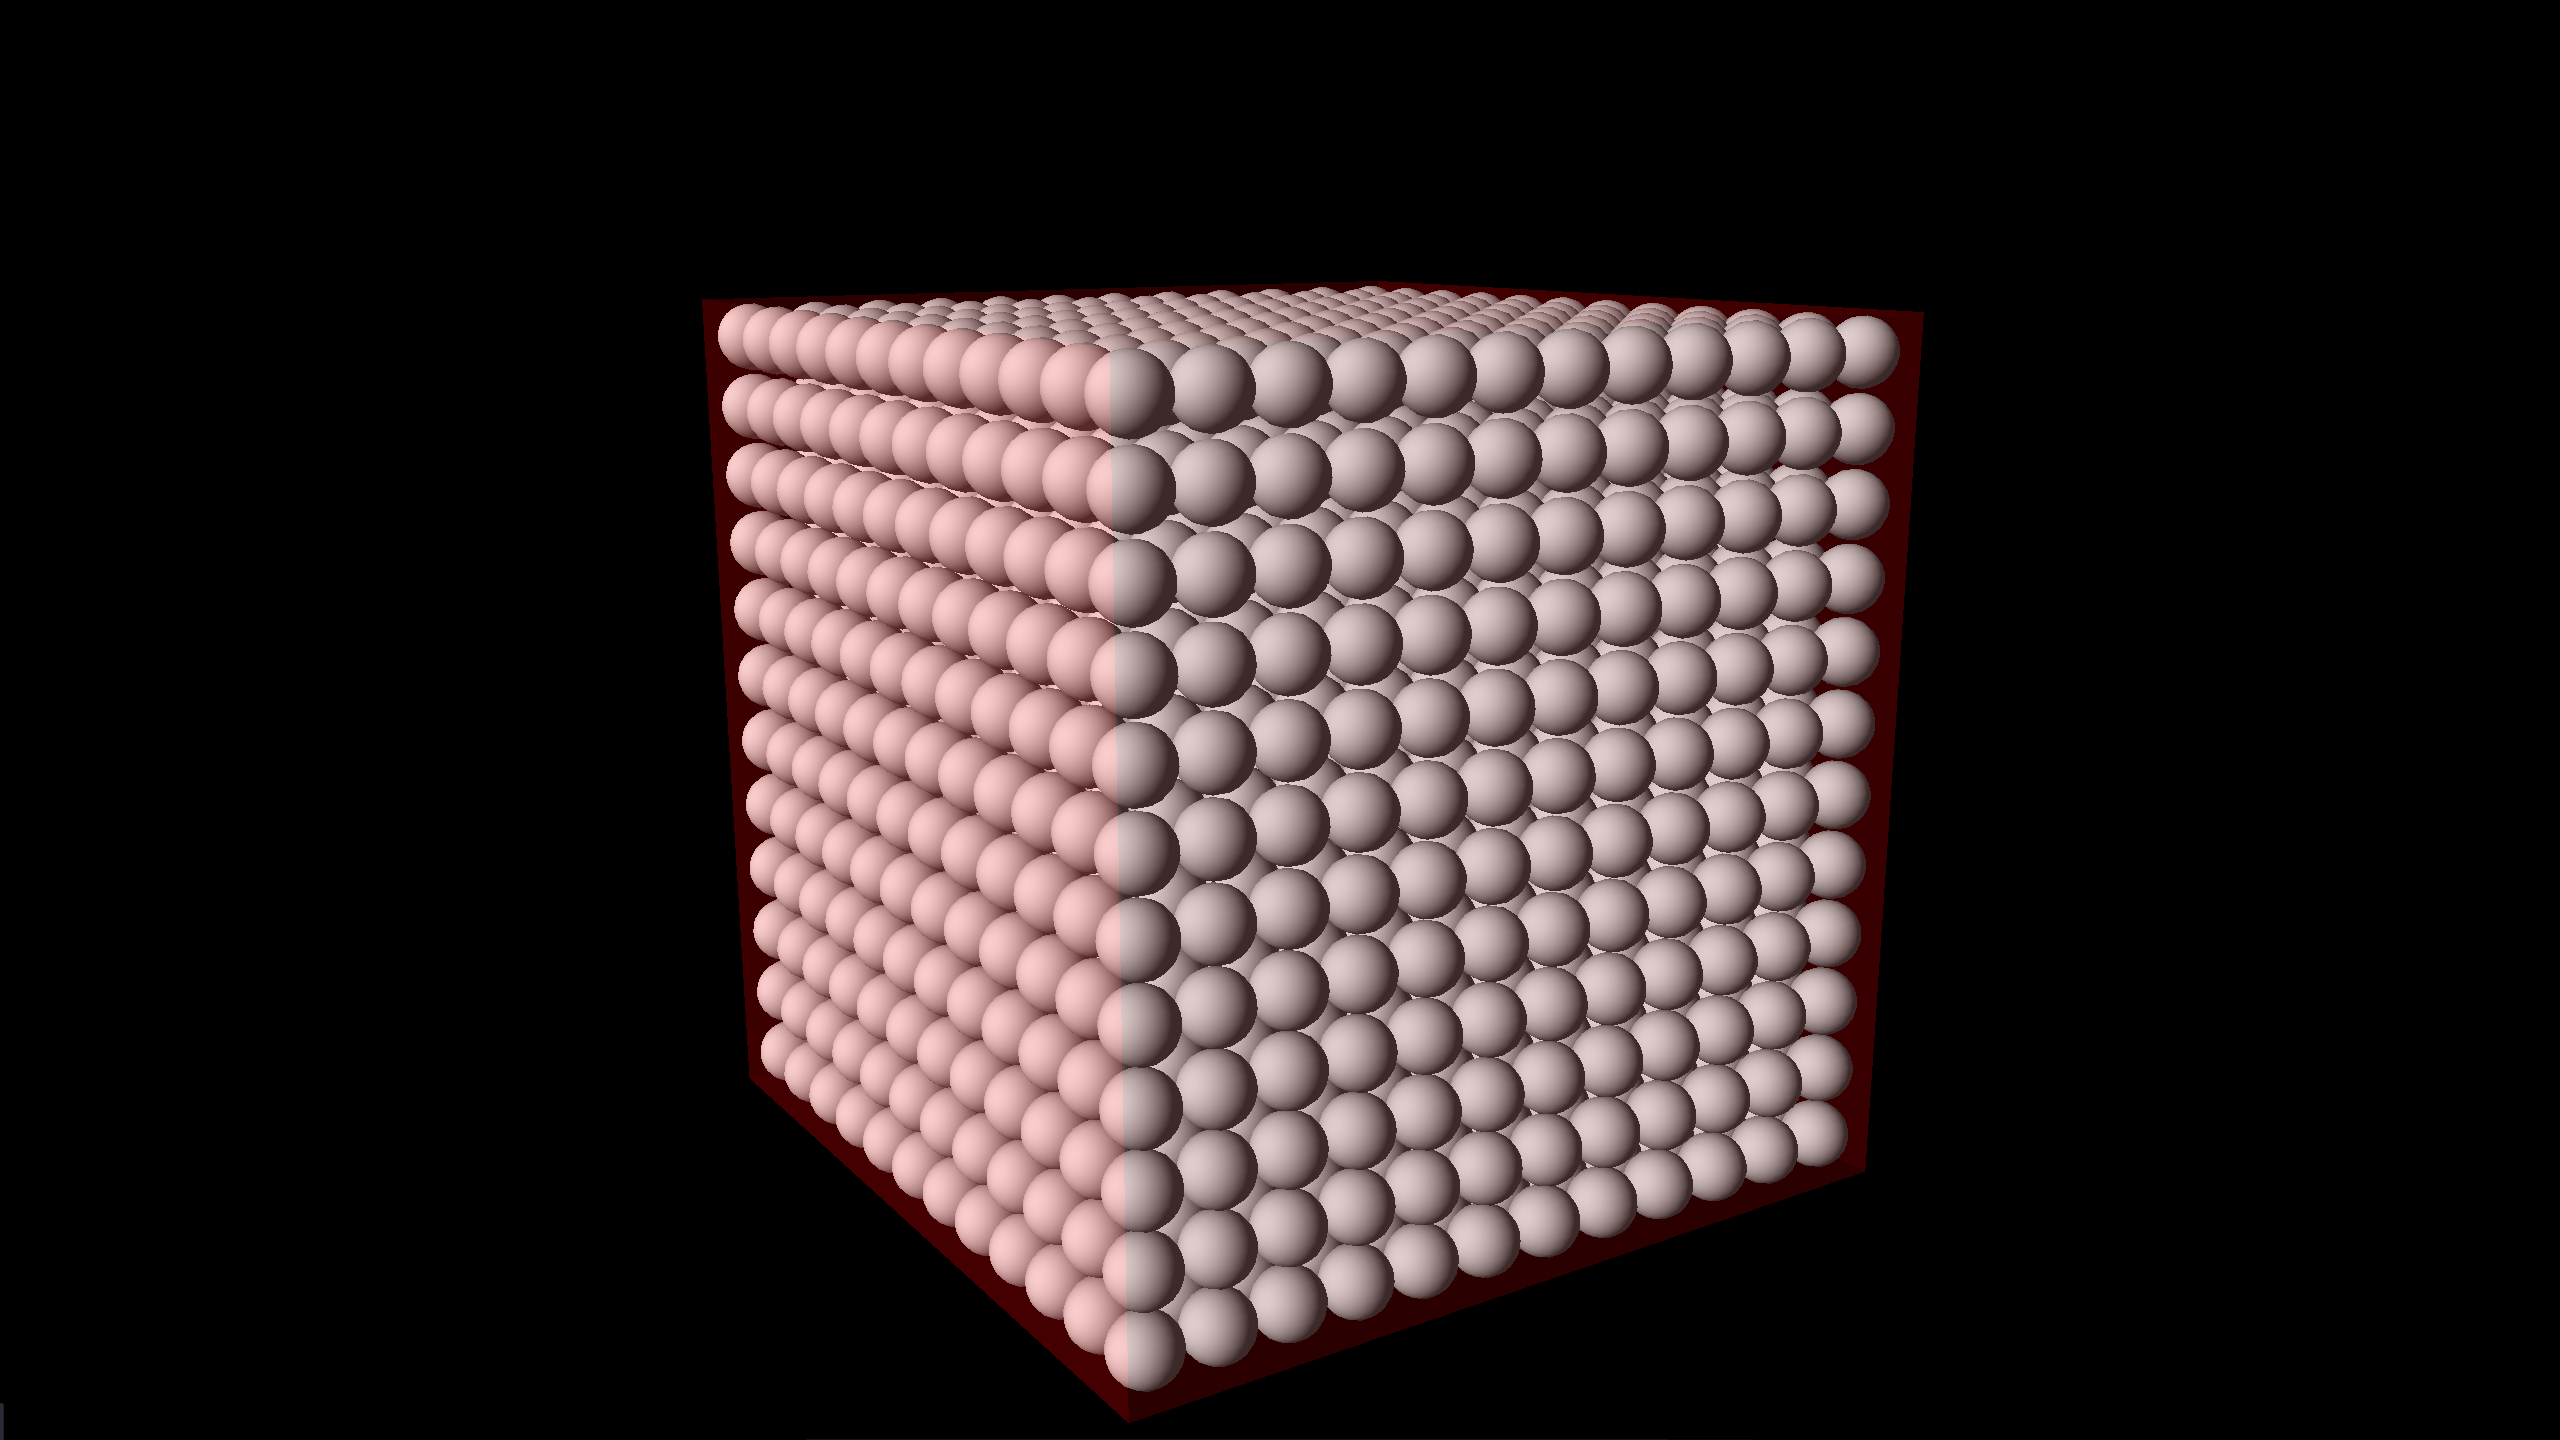
\includegraphics[width=0.45\textwidth]{../graphs/sc.png}
    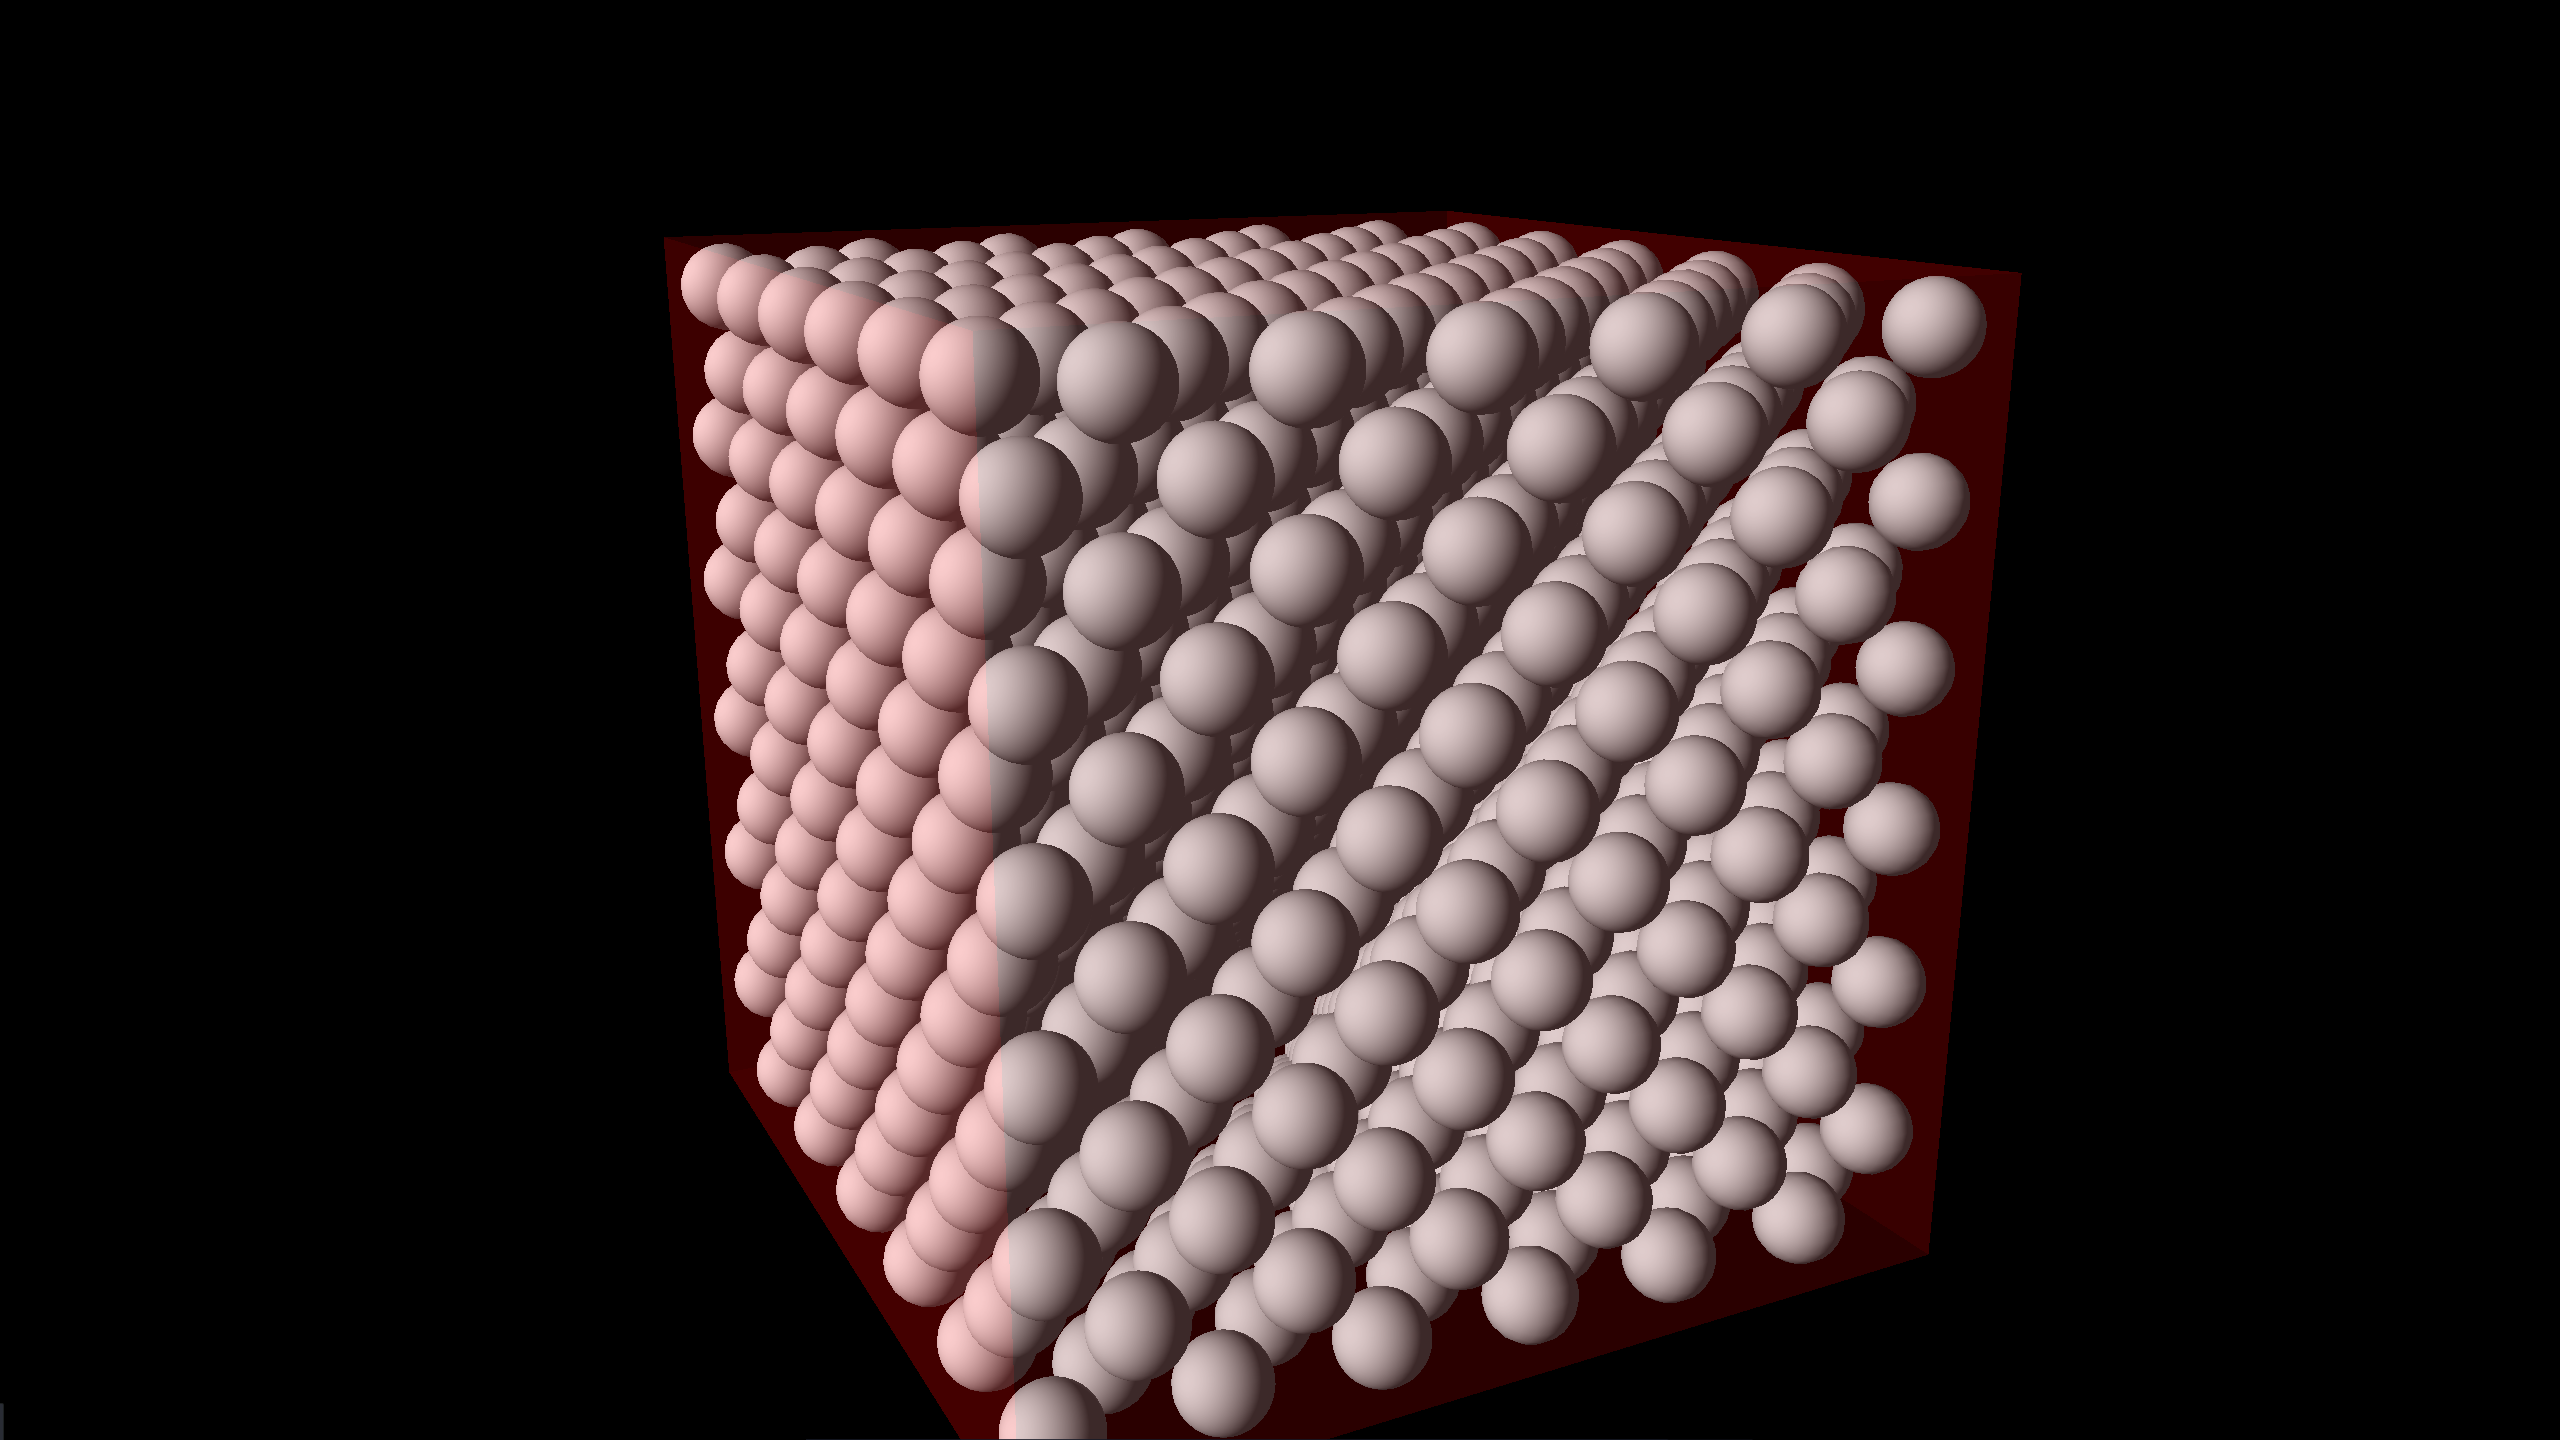
\includegraphics[width=0.45\textwidth]{../graphs/fcc.png}
    \caption{Graphical representation of an SC lattice (left) and a FCC lattice (right). Boundaries can be seen as a transparent red rectangle.}
  \end{center}
\end{figure}

As we did with the hexagonal lattice, we can now compute $\avg{R^2(\eta)}$ and determine $\eta_*$ of the transition. In the following plot this data is represented:

\begin{figure}[H]
  \begin{center}
    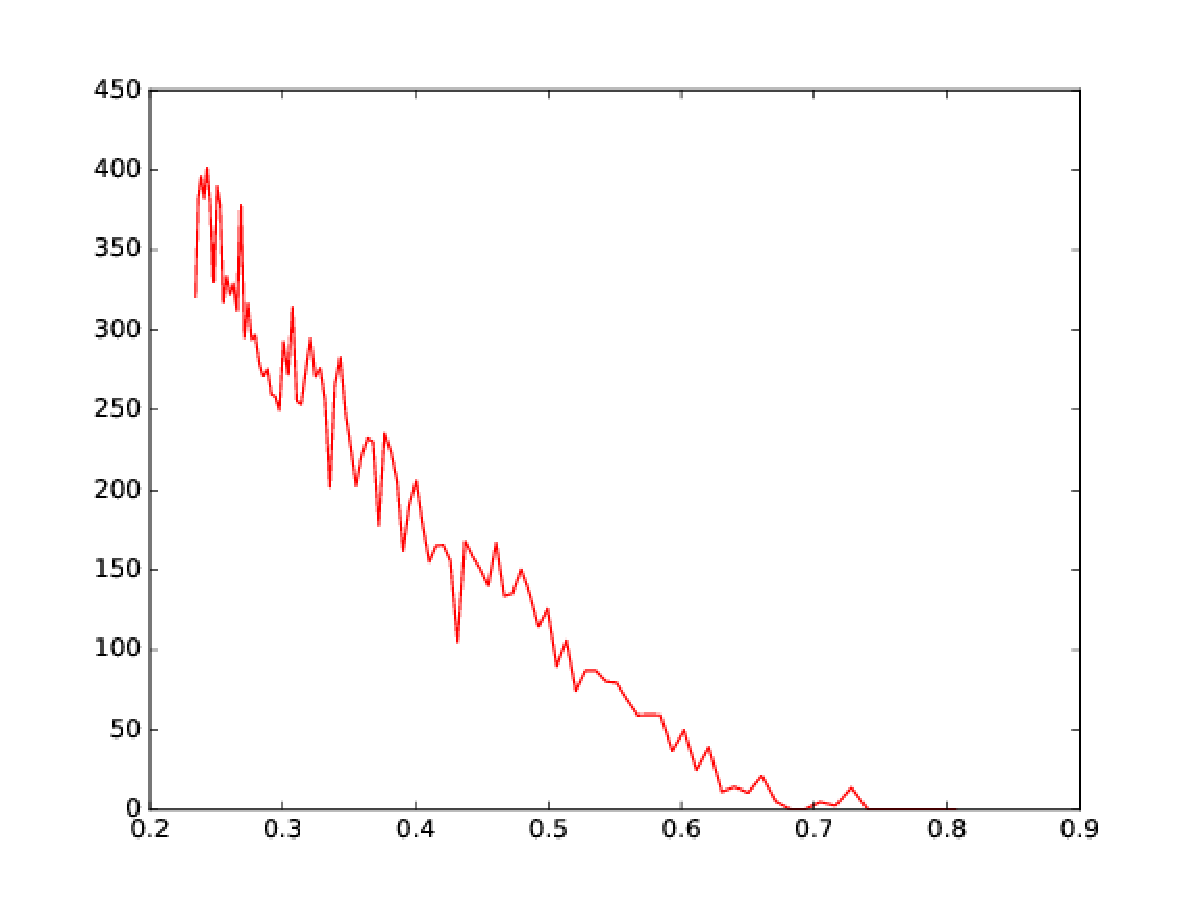
\includegraphics[width=0.7\textwidth]{../graphs/fcc-melting.pdf}
    \caption{Graphical representation of $\avg{R^2(\eta)}$ for an FCC lattice.}
  \end{center}
\end{figure}

In this case we find a value quite similar to the one for the hexagonal lattice, although there are more noise fluctuations so this value is not really precise. A better procedure would be to compute another average over multiple systems, so these fluctuations smooth out.

\section{Optimal step size}

Choosing a good value for $\Delta$ in the program is a great way to improve efficiency and accuracy, as not the same step size is useful for every system. We could say that a good trade-off $\Delta$ would be the one that keeps the number of hits and misses while moving particles balanced, or in other words, a fifty percent chance of acceptance $acc$.

There are various ways to achieve this, for example studying the system and plotting $acc(\Delta)$. However, in the program we have implemented a small function to adapt $\Delta$ in response to changes in $acc$.

Basically, to keep $acc \sim 0.5$, we multiply $\Delta$ times 0.9 when $acc < 0.4$ or times 1.1 when $acc > 0.5$, after computing $acc$ as the average of hits and misses in the previous steps.

\end{document}
